\begin{annexesenv}

% Imprime uma página indicando o início dos anexos
\partannexes

\chapter{INA 326 complete Schematic.}

\begin{figure}[!htpb]
  \centering
  \caption{INA 326 Complete Schematic}
  \label{INA-complete-schematic}
  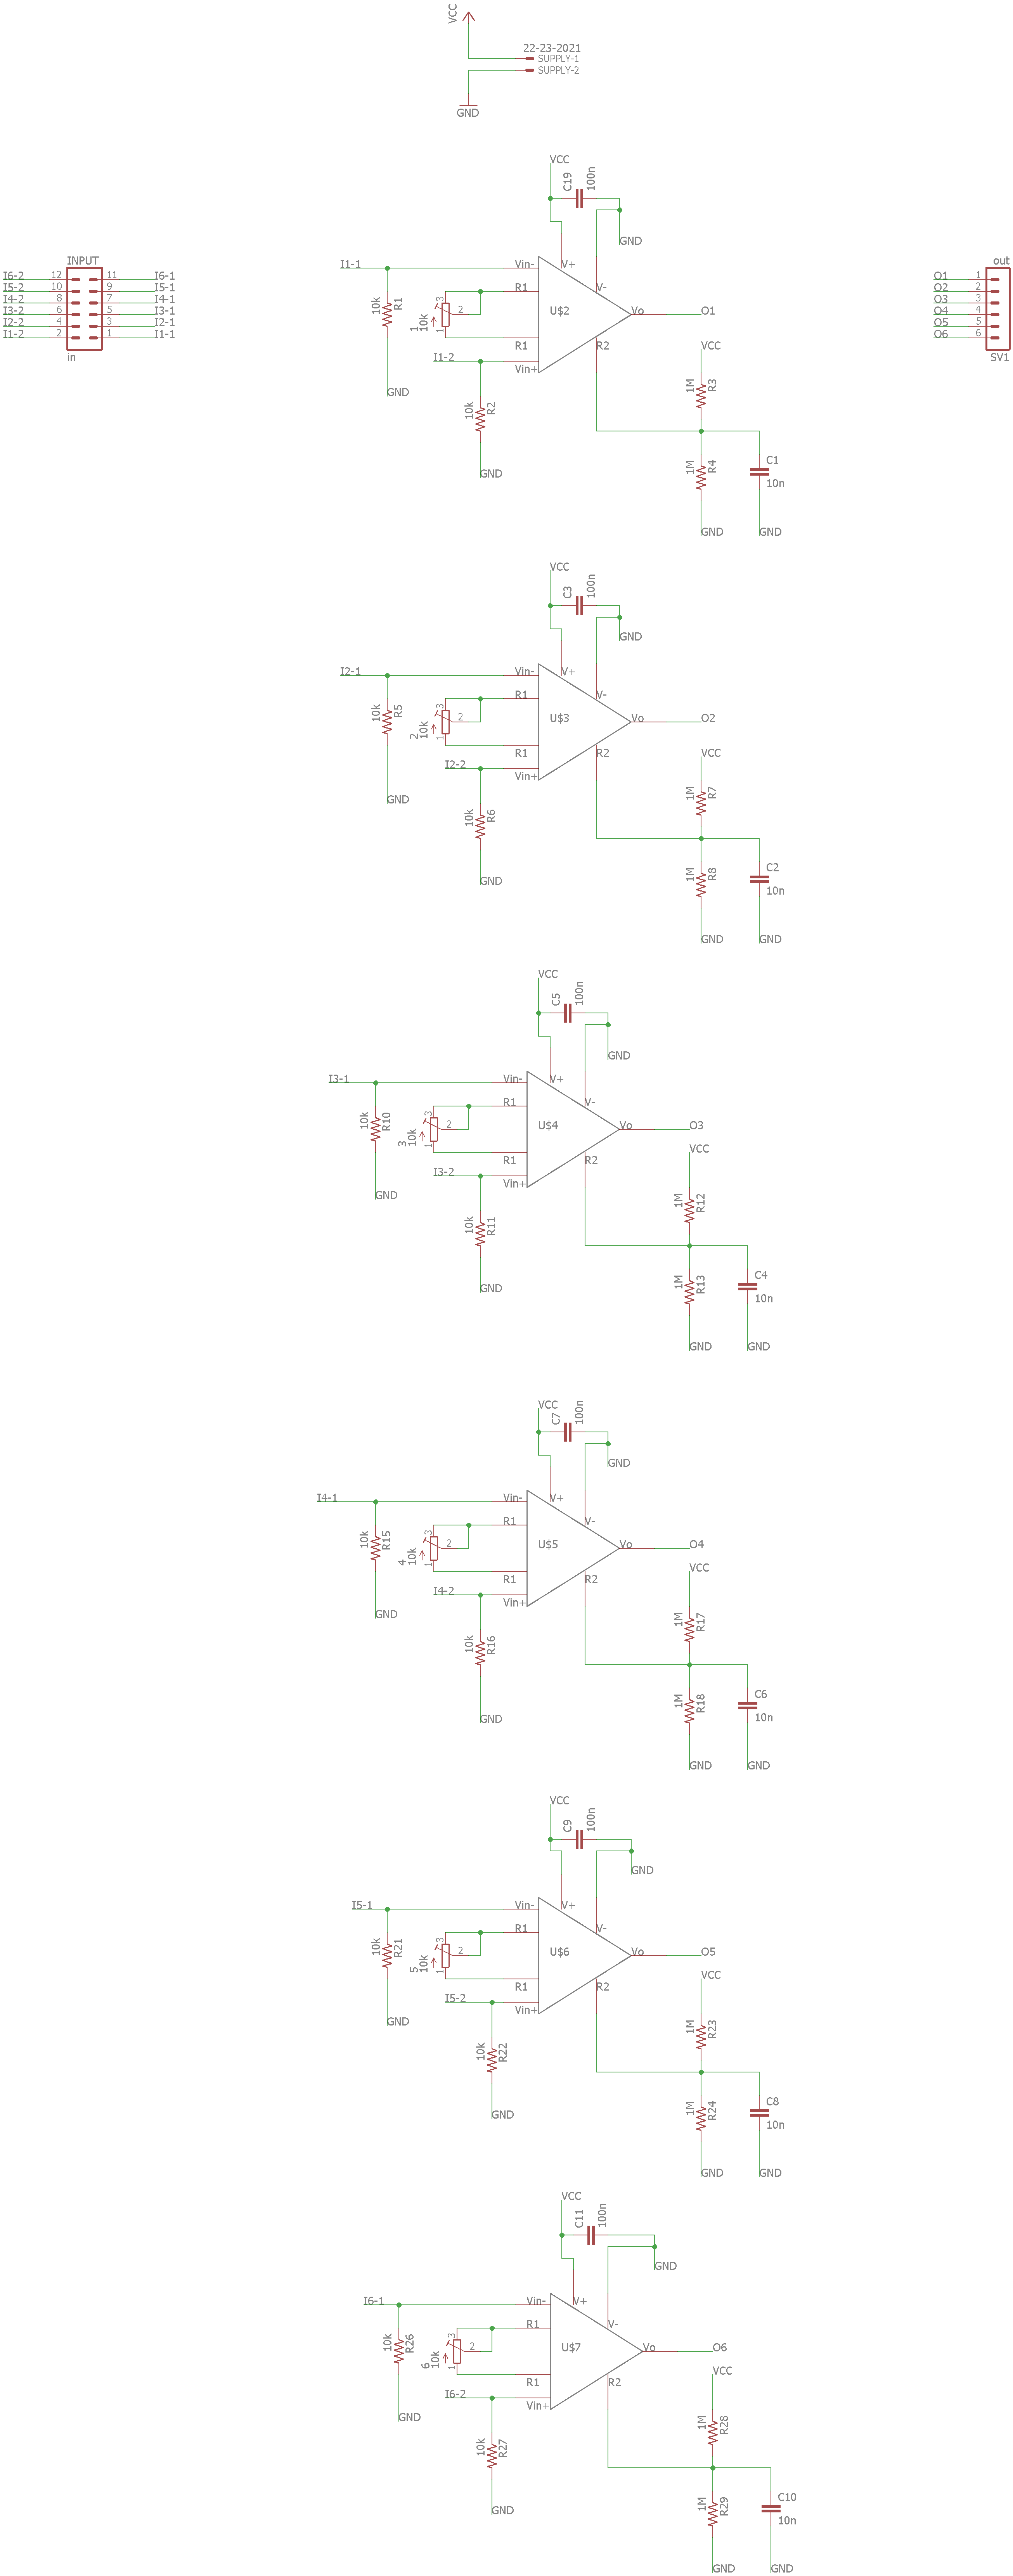
\includegraphics[scale=0.35]{images/INA/complete-schematic}
  \legend{Source: authors}
\end{figure}

\end{annexesenv}

\chapter{Prototype Cost Table.}

Costs are given on Brazilian Real.\\
\begin{table}[htb]
  \begin{center}
    \ABNTEXreducedfont
    \caption[Prototype Board Cost Table]{Prototype Board Cost Table}
    \label{Prototype-cost}
    \begin{tabular}{|c|c|c|}
      \hline
    Component & Quantity & Cost \\ \hline
    INA326 & 6 & 120.00\\ \hline
    10k$\Omega$ Trimmer Potentiometer & 6 & 7.50 \\ \hline
    10nF Ceramic Capacitor & 6 & 1.00 \\ \hline
    100nF Electrolytic Capacitor & 6 & 1.50 \\ \hline
    10k$\Omega$ Resistor 5$\%$ tolerancy & 12 & 2.00 \\ \hline
    1M$\Omega$ Resistor 5$\%$ tolerancy & 12 & 2.00 \\ \hline
    Pin bar 1x40 & 1 & 3.00 \\ \hline
    PCB & 2 & 50.00 \\ \hline
  \end{tabular}
  \legend{Source: authors}
\end{center}
\end{table}

\chapter{Production Cost Table.}

Costs are given on United States Dollar for production of 1000 samples.\\
\begin{table}[htb]
  \begin{center}
    \ABNTEXreducedfont
    \caption[Production Board Prediction Cost Table]{Production Board Prediction Cost Table}
    \label{Production-cost}
    \begin{tabular}{|c|c|c|c|}
      \hline
    Component & Quantity & Cost per Component & Total Cost \\ \hline
    INA326 & 6000 & 2.53071 & 15184.26\\ \hline
    10k$\Omega$ Trimmer Potentiometer & 6000 & 2.16050 & 12963.00 \\ \hline
    10nF Ceramic Capacitor & 6000 & 0.00233 & 13.98 \\ \hline
    100nF Electrolytic Capacitor & 6000 & 0.04431 & 265.86 \\ \hline
    10k$\Omega$ Resistor 1$\%$ tolerancy & 12000 & 0.00649 & 77.88 \\ \hline
    1M$\Omega$ Resistor 1$\%$ tolerancy & 12000 & 0.00671 & 80.52 \\ \hline
    Pin bar 1x40 & 1000 & 0.62240 & 622.40 \\ \hline
    PCB & 1000 & 0.22 & 223.94 \\ \hline
  \end{tabular}
  \legend{Source: \citeonline{Digikey} and \citeonline{PCB-maker} }
\end{center}
\end{table}
